% (C) 2024 Jie-Yin Lin and Yung-Yu Chen.  All rights reserved.
% chktex-file 3
% chktex-file 8
% chktex-file 10
% chktex-file 13
% chktex-file 17
% chktex-file 24
% chktex-file 25
% chktex-file 36
% chktex-file 37

\documentclass{turgon}
\usepackage[printwatermark]{xwatermark}
\usepackage{tikz}
\usetikzlibrary{shapes.geometric, arrows, positioning}
\newwatermark[allpages,color=black!15,angle=55,scale=5,xpos=0,ypos=0]%
{DRAFT}

\linespread{1.2}

\title{
%
Fit Four-digit NACA Airfoil with Cubic Bezier Curve
%
}

\author{
%
Jie-Yin Lin and Yung-Yu Chen
%
}

\begin{document}
\maketitle
\tableofcontents

%%%%%%%%%%%%%%%%%%%%%%%%%%%%%%%%%%%%%%%%%%%%%%%%%%%%%%%%%%%%%%%%%%%%%%%%%%
%%
\chapter*{Introduction}
\addcontentsline{toc}{chapter}{Introduction}
%%
%%%%%%%%%%%%%%%%%%%%%%%%%%%%%%%%%%%%%%%%%%%%%%%%%%%%%%%%%%%%%%%%%%%%%%%%%%

This file collects notes to fit NACA airfoil by using cubic Bezier curve so
that we can generate mesh for field to be solved by using the CESE
method\cite{chang_method_1995}.

%%%%%%%%%%%%%%%%%%%%%%%%%%%%%%%%%%%%%%%%%%%%%%%%%%%%%%%%%%%%%%%%%%%%%%%%%%
%%
\chapter{Four-digit NACA Airfoil}
% ref: https://en.wikipedia.org/wiki/NACA_airfoil#Five-digit_series
%%
%%%%%%%%%%%%%%%%%%%%%%%%%%%%%%%%%%%%%%%%%%%%%%%%%%%%%%%%%%%%%%%%%%%%%%%%%%

Terminology used for defining the airfoil:
\begin{enumerate}
    \item
    Chord ($c$)
    \item
    Maximum camber ($m$)
    \item
    Maximum camber location ($p$)
    \item
    Maximum thickness ($h$)
    \item
    Camber line (red dashed line)
    \item
    Leading edge ($x=0, y=0$)
    \item
    Trailing edge ($x=c, y=0$)
\end{enumerate}
\begin{figure}[h!]
    \centering
    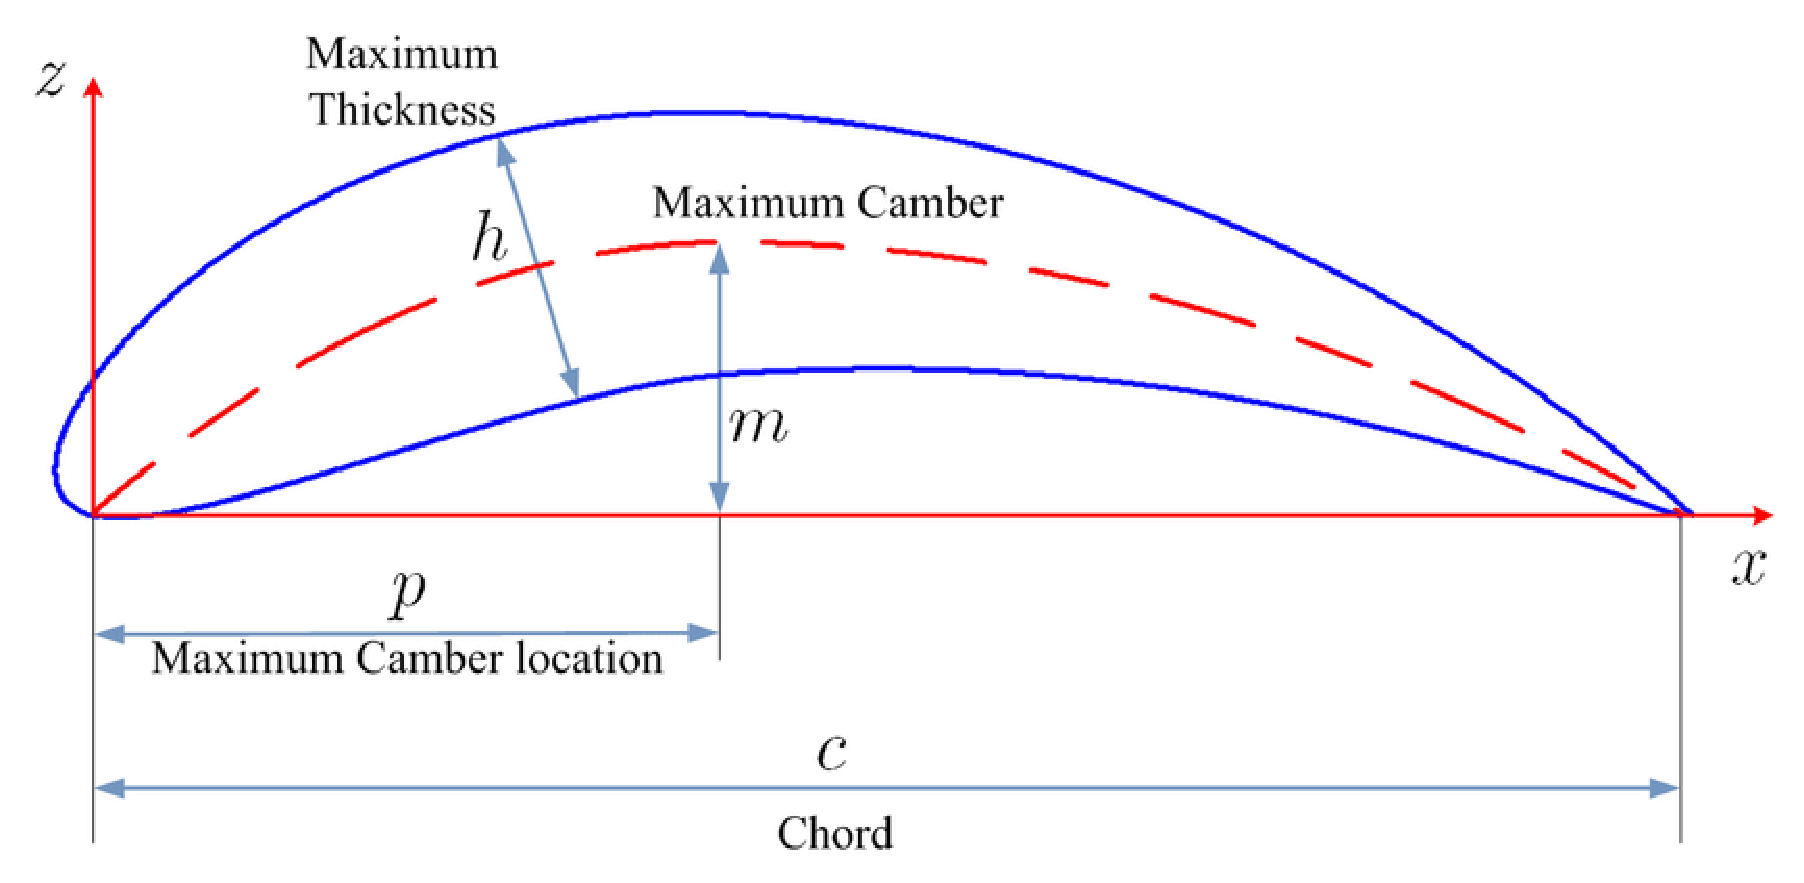
\includegraphics[width=0.5\textwidth]{airfoil_shape_image.eps}
    \caption{The parameters in wing profile.}
    \label{f:airfoil_shape_image}
\end{figure}
% figure downloaded from: https://www.researchgate.net/figure/AIRFOIL-SHAPE-PARAMETERS_fig4_267490031

The wing profile is defined by four-digit ($\mathrm{XYZZ}$):
\begin{enumerate}
    \item
    The 1st digit is the maximum camber as percentage of the chord.
    \begin{equation*}
        m = c \times (\mathrm{X}/100)
    \end{equation*}
    \item
    The 2nd digit is the maximum camber location in tenths of the chord.
    \begin{equation*}
        p = c \times (\mathrm{Y}/10)
    \end{equation*}
    \item
    The last two digits are the maximum thickness as percent of the chord.
    \begin{equation*}
        h = c \times (\mathrm{ZZ}/100)
    \end{equation*}
\end{enumerate}

The formula to calculate the thickness is
\begin{equation*}
    y_h = 5h\left( 0.2969\sqrt{x}-0.1260x-0.3516x^2+0.2843x^3-0.1015x^4 \right)
\end{equation*}
where $x$ is the position along the chord (from $0$ to $1$), $y_h$ is the
half thickness at a given value of $x$, and $h$ is the maximum thickness.

The camber line equation is
\begin{equation*}
    y_c =
    \begin{cases}
        \frac{m}{p^2} (2px - x^2); & 0 \leq x \leq p \\
        \frac{m}{(1 - p)^2} (1 - 2p + 2px - x^2); & p \leq x \leq 1
    \end{cases}
\end{equation*}
where $y_c$ is the camber line point at a given value of $x$, $m$ is the
maximum camber, and $p$ is the location of maximum camber.

The point $\mathbf{F}_u(x)$ in upper surface equation is
\begin{equation}
    \mathbf{F}_u(x) =
    \begin{bmatrix}
        x_u \\ y_u
    \end{bmatrix}
    =
    \begin{bmatrix}
        x - y_h \sin\theta \\ y_c + y_h \cos\theta
    \end{bmatrix}
    \label{e:naca:up_xy}
\end{equation}
and the point $\mathbf{F}_l(x)$ in lower surface equation is
\begin{equation*}
    \mathbf{F}_l(x) =
    \begin{bmatrix}
        x_u \\ y_u
    \end{bmatrix}
    =
    \begin{bmatrix}
        x + y_h \sin\theta \\ y_c - y_h \cos\theta
    \end{bmatrix}
\end{equation*}
where
\begin{equation*}
    \arctan \theta =
    \begin{cases}
        \frac{2m}{p^2} (p - x); & 0 \leq x \leq p \\
        \frac{2m}{(1 - p)^2} (p - x); & p \leq x \leq 1
    \end{cases}
\end{equation*}

%%%%%%%%%%%%%%%%%%%%%%%%%%%%%%%%%%%%%%%%%%%%%%%%%%%%%%%%%%%%%%%%%%%%%%%%%%
%%
\chapter{Cubic Bezier Curve}
% ref: https://en.wikipedia.org/wiki/Bernstein_polynomial
% ref: https://en.wikipedia.org/wiki/B%C3%A9zier_curve#Cubic_B%C3%A9zier_curves
%%
%%%%%%%%%%%%%%%%%%%%%%%%%%%%%%%%%%%%%%%%%%%%%%%%%%%%%%%%%%%%%%%%%%%%%%%%%%

The basis functions for an $n$th degree Bezier curve are expressed as a linear
combination of Bernstein basis polynomials of degree $n$.

\begin{figure}[h!]
    \centering
    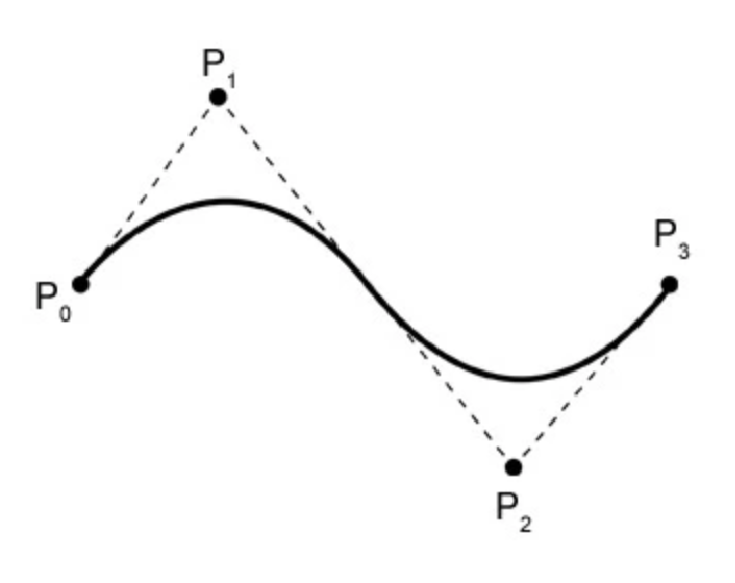
\includegraphics[width=0.3\textwidth]{cubic_bezier_curve.eps}
    \caption{The cubic Bezier curve.}
    \label{f:cubic_bezier_curve}
\end{figure}
% figure downloaded from: https://btnseniorproject17.wordpress.com/2017/05/01/more-unity-part-2-path-following-and-bezier-curves/

The items of Bernstein basis polynomials of degree $n$ are defined as
\begin{equation}
    b_{m, n}(t) = {n \choose m} t^m (1 - t)^{n - m}
    \label{e:cbc:bbp}
\end{equation}
where ${n \choose m}$ is a binomial coefficient and $m = 0, 1, \dots, n$. The
Bernstein basis polynomials have the following properties:
\begin{enumerate}
    \item
    $b_{m, n}(t) = 0$, if $m < 0$ or $m > n$.
    \item
    $b_{m, n}(t) \geq 0$, for $t \in [0, 1]$.
    \item
    $b_{m, n}(1 - t) = b_{n - m, n}(t)$.
\end{enumerate}
The cubic Bezier curve is defined by 4 control points $\mathbf{P}_i$,
$i = 0, 1, 2, 3$:
\begin{equation*}
    \mathbf{P}_i =
    \begin{bmatrix}
        P_{xi} \\ P_{yi}
    \end{bmatrix}
\end{equation*}
The function $\mathbf{B}(t)$ is
\begin{equation*}
    \mathbf{B}(t) = \Sigma b_{i,3}(t)\mathbf{P}_i
\end{equation*}
where $b_{i,3}(t)$ is shown in Eq.~(\ref{e:cbc:bbp}). This function can be
expanded to
\begin{equation}
    \mathbf{B}(t) = (1-t)^3 \mathbf{P}_0 + 3(1-t)^2 t \mathbf{P}_1 + 3(1-t) t^2 \mathbf{P}_2 + t^3 \mathbf{P}_3
    \label{e:cbc:der0}
\end{equation}
where $0 \leq t \leq 1$. The first-order derivative of $\mathbf{B}(t)$ is
\begin{equation*}
    \mathbf{B}^\prime(t) = 3 \left[
        (1-t)^2 (\mathbf{P}_1 - \mathbf{P}_0) + 2(1-t)t(\mathbf{P}_2 - \mathbf{P}_1) + t^2(\mathbf{P}_3 - \mathbf{P}_2)
    \right]
\end{equation*}
The second-order derivative of $B(t)$ is
\begin{equation*}
    \mathbf{B}^{\prime \prime}(t) = 6 \left[ (1-t)(\mathbf{P}_2 - 2\mathbf{P}_1 +\mathbf{P}_0) + t(\mathbf{P}_3 - 2\mathbf{P}_2 + \mathbf{P}_1) \right]
\end{equation*}

For a sequence of $n$ cubic Bezier curves, $\mathbf{B}_0(t)$ through $\mathbf{B}_{n-1}(t)$,
there are $4n$ control points can be adjusted. It implies that there
are $4n$ dimensions of freedom. Assume the first and last points are
fixed. If we wish the value, slope, and curvature between any two Bezier
curves are continuous, the degree of freedom will become $n+1$. Thus, we
can keep the continuous value of curvature when adding the number of Bezier
curves.

%%%%%%%%%%%%%%%%%%%%%%%%%%%%%%%%%%%%%%%%%%%%%%%%%%%%%%%%%%%%%%%%%%%%%%%%%%
%%
\chapter{Levenberg-Marquardt Algorithm}
% ref: https://en.wikipedia.org/wiki/Levenberg%E2%80%93Marquardt_algorithm
%%
%%%%%%%%%%%%%%%%%%%%%%%%%%%%%%%%%%%%%%%%%%%%%%%%%%%%%%%%%%%%%%%%%%%%%%%%%%

Levenberg-Marquardt algorithm (LM) is used to solve non-linear least
squares problems, especailly for curve fitting. The LM combines
Gauss-Newton algorithm and gradient descent algorithm. It can find the
solution efficiently even if the initial point is set undesirably.

For a non-linear least squares curve fitting problem, the sum of the
squares of the deviations $S(\beta)$ is
\begin{equation}
    \label{e:lm:sd}
    S(\beta) = \sum_{i=1}^N \left| y_i - f(x_i, \beta) \right|^2
\end{equation}
where $f(x, \beta)$ is a curve function, and $(x_i, y_i)$ is a set of $N+$
empirical pairs. To replace $\beta$ with $\beta + \delta$, the function
$f(x_i, \beta + \delta)$ is approximated by linearization
\begin{equation}
    f(x_i, \beta + \delta) \approx f(x_i, \beta) + J_i \delta
    \label{e:lm:f_apx}
\end{equation}
where $J_i$ is the gradient of $f$ with respect to $\beta$
\begin{equation*}
    J_i = \frac{\partial f(x_i, \beta)}{\partial \beta}
\end{equation*}
To get the $S(\beta + \delta)$, substitute Eq.~(\ref{e:lm:f_apx}) into
Eq.~(\ref{e:lm:sd}) in vector notation
\begin{equation*}
    S(\beta + \delta) \approx
    \left| \mathbf{y} - \mathbf{f}(\beta) - \mathbf{J} \mathbf{\delta} \right|^2
\end{equation*}
where $\mathbf{J}$ is the Jacobian matrix, whose $i$th row is $J_i$. Set
the derivative of $S(\beta + \delta)$ with respect to $\delta$ as zero to
get the solution for minimizing $S(\beta + \delta)$
\begin{equation*}
    \left( \mathbf{J}^\top \mathbf{J} \right) \mathbf{\delta} =
    \mathbf{J}^\top \left[ \mathbf{y} - \mathbf{f}(\beta) \right]
\end{equation*}
Levenberg adds a damping term to make it become
\begin{equation*}
    \left( \mathbf{J}^\top \mathbf{J} + \lambda \mathbf{I} \right)
    \mathbf{\delta} =
    \mathbf{J}^\top \left[ \mathbf{y} - \mathbf{f}(\beta) \right]
\end{equation*}
where $\mathbf{I}$ is the identity matrix. And the $\delta$ can be sloved as
\begin{equation}
    \mathbf{\delta} = \left( \mathbf{J}^\top \mathbf{J} + \lambda \mathbf{I} \right)^{-1}
    \mathbf{J}^\top \left[ \mathbf{y} - \mathbf{f}(\beta) \right]
    \label{e:lm:sol}
\end{equation}
If $\lambda \rightarrow 0$, the LM becomes Gauss-Newton algorithm. And, if
$\lambda \rightarrow \infty$, the LM becomes gradient descent algorithm.

The general flow chart in LM:
\tikzstyle{rect} = [rectangle, text width = 5cm, minimum height = 0.7cm, draw = black, text centered]
\tikzstyle{diam} = [diamond, text width = 2.2cm, minimum height = 0.7cm, draw = black, text centered]
\tikzstyle{arrow} = [thick, ->, >=stealth]
\begin{figure}[h!]
    \centering
    \begin{tikzpicture}[node distance = 0.7cm, font = \small]
        \node (rect_seb0) [rect] {Set $\beta$ = $\beta_0$.};
        \node (rect_cps0) [rect, below = of rect_seb0] {Compute $S_0(\beta)$.};
        \node (diam_chk0) [diam, below = of rect_cps0] {$S_0 < \epsilon$ ?};
        \node (rect_sel1) [rect, below = of diam_chk0] {Set $\lambda_1$ = $\lambda_0$.};
        \node (rect_seb1) [rect, below = of rect_sel1] {Solve $\delta(\lambda_1)$ and $\beta$ = $\beta$ + $\delta$.};
        \node (rect_cps1) [rect, below = of rect_seb1] {Compute $S_1(\beta)$.};
        \node (diam_chk1) [diam, below = of rect_cps1] {$S_1 < \epsilon$ ?};
        \node (rect_sel2) [rect, below = of diam_chk1] {Set $\lambda_2$ = $\lambda_1/\nu$.};
        \node (rect_seb2) [rect, below = of rect_sel2] {Solve $\delta(\lambda_2)$ and $\beta$ = $\beta$ + $\delta$.};
        \node (rect_cps2) [rect, below = of rect_seb2] {Compute $S_2(\beta)$.};
        \node (diam_chk2) [diam, below = of rect_cps2] {$S_2 < \epsilon$ ?};
        \node (rect_solu) [rect, below = of diam_chk2] {Get $\beta$.};
        \node (diam_cmp2) [diam, right of = diam_chk2, xshift=4cm] {$S_2 < S_0, S_1$ ?};
        \node (diam_cmp1) [diam, right of = diam_cmp2, xshift=4cm] {$S_1 < S_0$ ?};
        \node (rect_rsl2) [rect, right of = rect_seb2, xshift=8.7cm] {Set $\lambda_2$ = $\lambda_1$.};
        \node (rect_rsl1) [rect, right of = rect_seb1, xshift=8.7cm] {Set $\lambda_1$ = $\lambda_2$.};
        \draw [arrow] (rect_seb0) -- (rect_cps0);
        \draw [arrow] (rect_cps0) -- (diam_chk0);
        \draw [arrow] (diam_chk0.west) node[anchor = south east]{Yes} -| ++(-2, 0) |- (rect_solu);
        \draw [arrow] (diam_chk0.south) node[anchor = north west]{No} -- (rect_sel1);
        \draw [arrow] (rect_sel1) -- (rect_seb1);
        \draw [arrow] (rect_seb1) -- (rect_cps1);
        \draw [arrow] (rect_cps1) -- (diam_chk1);
        \draw [arrow] (diam_chk1.west) node[anchor = south east]{Yes} -| ++(-2, 0) |- (rect_solu);
        \draw [arrow] (diam_chk1.south) node[anchor = north west]{No} -- (rect_sel2);
        \draw [arrow] (rect_sel2) -- (rect_seb2);
        \draw [arrow] (rect_seb2) -- (rect_cps2);
        \draw [arrow] (rect_cps2) -- (diam_chk2);
        \draw [arrow] (diam_chk2.south) node[anchor = north west]{Yes} -- (rect_solu);
        \draw [arrow] (diam_chk2.east) node[anchor = south west]{No} -- (diam_cmp2);
        \draw [arrow] (diam_cmp2.north) node[anchor = south west]{Yes} |- (rect_seb2);
        \draw [arrow] (diam_cmp2.east) node[anchor = south west]{No} -- (diam_cmp1);
        \draw [arrow] (diam_cmp1.north) node[anchor = south west]{Yes} -- (rect_rsl2);
        \draw [arrow] (diam_cmp1.east) node[anchor = south west]{No} -| ++(2, 0) |- (rect_rsl1);
        \draw [arrow] (rect_rsl2) -- (rect_seb2);
        \draw [arrow] (rect_rsl1) -- (rect_seb1);
    \end{tikzpicture}
    \caption{The flow chart of LM.}
    \label{f:lm_flow_chart}
\end{figure}

In the LM flow, $\beta_0$, $\lambda_0$, $\epsilon$, and $\nu$ have to be
decided. $\epsilon$ is the error tolerance, and $\nu$ is a constant greater
than 1.

%%%%%%%%%%%%%%%%%%%%%%%%%%%%%%%%%%%%%%%%%%%%%%%%%%%%%%%%%%%%%%%%%%%%%%%%%%
%%
\chapter{Linear Least Squares}
% ref: https://en.wikipedia.org/wiki/Linear_least_squares
%%
%%%%%%%%%%%%%%%%%%%%%%%%%%%%%%%%%%%%%%%%%%%%%%%%%%%%%%%%%%%%%%%%%%%%%%%%%%

Linear least squares (LLS) is a set of formulations for solving statistical
problems involved in linear regression, including variants for ordinary,
weighted, and generalized residuals.

Consider the linear equation
\begin{equation}
    \mathbf{A} \mathbf{x} = \mathbf{b}
    \label{e:lls:leq}
\end{equation}
where $\mathbf{A} \in \mathbb{R}^{m \times n}$ and $\mathbf{b} \in \mathbb{R}^m$. When $m>n$,
$\mathbf{x} \in \mathbb{R}^n$ is the solution of
\begin{equation*}
    \underset{\mathbf{x} \in \mathbb{R}^n}{\text{minimize}} \left| \mathbf{A} \mathbf{x} - \mathbf{b} \right|^2
\end{equation*}
$\mathbf{x}$ can be computed by
\begin{equation*}
    \mathbf{A}^\top \mathbf{A} \mathbf{x}^* = \mathbf{A}^\top \mathbf{b}
\end{equation*}
\begin{equation}
    \mathbf{x}^* = (\mathbf{A}^\top \mathbf{A})^{-1} \mathbf{A}^\top \mathbf{b}
    \label{e:lls:sol}
\end{equation}
where $\mathbf{A}^\top$ denotes the transpose of $\mathbf{A}$ and $\mathbf{A} \mathbf{x}^*$ is the projection of
$\mathbf{b}$ in columnn space of $\mathbf{A}$.

%%%%%%%%%%%%%%%%%%%%%%%%%%%%%%%%%%%%%%%%%%%%%%%%%%%%%%%%%%%%%%%%%%%%%%%%%%
%%
\chapter{Fit Airfoil with Cubic Bezier Curve}
%%
%%%%%%%%%%%%%%%%%%%%%%%%%%%%%%%%%%%%%%%%%%%%%%%%%%%%%%%%%%%%%%%%%%%%%%%%%%

We define a function $S(\mathbf{P})$ as the sum of distance between cubic
Bezier curve point $\mathbf{B}(t_i, \mathbf{P})$ and 4-digut NACA airfoil
point $\mathbf{F}(x_i)$:
\begin{equation*}
    S(\mathbf{P}) = \sum_{i=1}^N \left|
        \mathbf{F}(x_i) - \mathbf{B}(t_i, \mathbf{P}) \right|^2 =
    \left[ \mathbf{F} - \mathbf{B}(\mathbf{P}) \right]^\top
    \left[ \mathbf{F} - \mathbf{B}(\mathbf{P}) \right]
\end{equation*}
where $\mathbf{F}$ is:
\begin{equation*}
    \mathbf{F} =
    \begin{bmatrix}
        x_0 \\ y_0 \\ x_1 \\ y_1 \\ \vdots \\ x_{N-1} \\ y_{N-1}
    \end{bmatrix}
\end{equation*}
where $x_i$ and $y_i$ are $x_u(x_i)$ and $y_u(x_i)$ in
Eq.~(\ref{e:naca:up_xy}). And then, $\mathbf{P}$ and
$\mathbf{B}(\mathbf{P})$ are:
\begin{equation*}
    \mathbf{P} =
    \begin{bmatrix}
        P_{x0} \\ P_{y0} \\ P_{x1} \\ P_{y1} \\
        P_{x2} \\ P_{y2} \\ P_{x3} \\ P_{y3}
    \end{bmatrix}
\end{equation*}
\begin{equation*}
    \mathbf{B}(\mathbf{P}) =
    \begin{bmatrix}
        \Sigma b_{i,3}(t_0)P_{xi} \\
        \Sigma b_{i,3}(t_0)P_{yi} \\
        \Sigma b_{i,3}(t_1)P_{xi} \\
        \Sigma b_{i,3}(t_1)P_{yi} \\
        \vdots \\
        \Sigma b_{i,3}(t_{N-1})P_{xi} \\
        \Sigma b_{i,3}(t_{N-1})P_{yi} \\
    \end{bmatrix}
\end{equation*}

Here, we fix $\mathbf{P}_0$ and $\mathbf{P}_3$ at leading edge and trailing
edge. By keeping $S(\mathbf{P})$, $\mathbf{B}(t_i, \mathbf{P})$,
$\mathbf{P}$, and $\mathbf{F}(x_i)$ can be rewritten as:
\begin{equation*}
    \mathbf{F} =
    \begin{bmatrix}
        x_0 - b_{0,3}(t_0)P_{x0} - b_{3,3}(t_0)P_{x3} \\
        y_0 - b_{0,3}(t_0)P_{y0} - b_{3,3}(t_0)P_{y3} \\
        x_1 - b_{0,3}(t_1)P_{x0} - b_{3,3}(t_1)P_{x3} \\
        y_1 - b_{0,3}(t_1)P_{y0} - b_{3,3}(t_1)P_{y3} \\
        \vdots \\
        x_{N-1} - b_{0,3}(t_{N-1} )P_{x0} - b_{3,3}(t_{N-1} )P_{x3} \\
        y_{N-1} - b_{0,3}(t_{N-1} )P_{y0} - b_{3,3}(t_{N-1} )P_{y3} 
    \end{bmatrix}
\end{equation*}
\begin{equation*}
    \mathbf{P} =
    \begin{bmatrix}
        P_{x1} \\ P_{y1} \\ P_{x2} \\ P_{y2}
    \end{bmatrix}
\end{equation*}
\begin{equation*}
    \mathbf{B}(\mathbf{P}) =
    \begin{bmatrix}
        b_{1,3}(t_0)P_{x1} + b_{2,3}(t_0)P_{x2} \\
        b_{1,3}(t_0)P_{y1} + b_{2,3}(t_0)P_{y2} \\
        b_{1,3}(t_1)P_{x1} + b_{2,3}(t_1)P_{x2} \\
        b_{1,3}(t_1)P_{y1} + b_{2,3}(t_1)P_{y2} \\
        \vdots \\
        b_{1,3}(t_{N-1})P_{x1} + b_{2,3}(t_{N-1})P_{x2} \\
        b_{1,3}(t_{N-1})P_{y1} + b_{2,3}(t_{N-1})P_{y2} \\
    \end{bmatrix}
\end{equation*}
For computing $S(\mathbf{P})$, a common way is to select the same location
of points at both $\mathbf{F}(x_i)$ and $\mathbf{B}(t_i, \mathbf{P})$.
Unfortunately, the distribution of $\mathbf{B}(t_i, \mathbf{P})$ is also
based on $\mathbf{P}$. It implies that this is a non-linear curve fitting
problem.

A general method to solve the non-linear least square problem is
Levenberg-Marquardt algorithm (LM). According to this problem, the
parameters $y_i$, $\beta$, and $f(x_i, \beta)$, in LM are equal to
$\mathbf{F}(x_i)$, $\mathbf{P}$, and $\mathbf{B}(t_i, \mathbf{P})$,
respectively. Also, $\mathbf{J}(t_i, \mathbf{P})$ can be computed:
\begin{equation*}
    \mathbf{J}(t_i, \mathbf{P}) =
    \frac{\partial \mathbf{B}(t_i, \mathbf{P})}{\partial \mathbf{P}} =
    \begin{bmatrix}
        b_{1,3}(t_i) & 0 & b_{2,3}(t_i) & 0 \\
        0 & b_{1,3}(t_i) & 0 & b_{2,3}(t_i)
    \end{bmatrix}
\end{equation*}
and the Jacobian matrix $\mathbf{J}(\mathbf{P})$ is:
\begin{equation*}
    \mathbf{J}(\mathbf{P}) =
    \begin{bmatrix}
        b_{1,3}(t_0) & 0 & b_{2,3}(t_0) & 0 \\
        0 & b_{1,3}(t_0) & 0 & b_{2,3}(t_0) \\
        b_{1,3}(t_1) & 0 & b_{2,3}(t_1) & 0 \\
        0 & b_{1,3}(t_1) & 0 & b_{2,3}(t_1) \\
        \vdots & \vdots & \vdots & \vdots \\
        b_{1,3}(t_{N-1}) & 0 & b_{2,3}(t_{N-1}) & 0 \\
        0 & b_{1,3}(t_{N-1}) & 0 & b_{2,3}(t_{N-1})
    \end{bmatrix}
\end{equation*}
After determining all parameters in LM, we can follow the LM flow chart in
Fig.~(\ref{f:lm_flow_chart}) to solve it. In the first step, the initial
$\mathbf{P}_1$ is set as the intersection point of tangent line at
$\mathbf{P}_0$ and tangent line at maximum thickness location, and
$\mathbf{P}_2$ is set as the intersection point of tangent line at
$\mathbf{P}_3$ and tangent line at maximum thickness location.

Aside from LM, linear least square (LLS) is also a method to solve curve
fitting problem. The parameters $\mathbf{A}$, $\mathbf{x}$, and
$\mathbf{b}$ are equal to $\mathbf{J}(\mathbf{P})$, $\mathbf{P}$, and
$\mathbf{F}$ in LM, respectively. And then, we design the flow using LLS:
\tikzstyle{rect} = [rectangle, text width = 5cm, minimum height = 0.7cm, draw = black, text centered]
\tikzstyle{diam} = [diamond, text width = 2.5cm, minimum height = 0.7cm, draw = black, text centered]
\tikzstyle{arrow} = [thick, ->, >=stealth]
\begin{figure}
    \centering
    \begin{tikzpicture}[node distance = 0.7cm, font = \small]
        \node (rect_cpb) [rect] {Compute $\mathbf{b}$.};
        \node (rect_sep) [rect, below = of rect_cpb] {Set $\mathbf{x}_0$.};
        \node (rect_cpa) [rect, below = of rect_sep] {Compute $\mathbf{A}(\mathbf{x}_0)$.};
        \node (rect_sox) [rect, below = of rect_cpa] {Solve $\mathbf{x}$.};
        \node (diam_chk) [diam, below = of rect_sox] {$\left| \mathbf{x} - \mathbf{x}_0 \right| < \epsilon$ ?};
        \node (rect_sol) [rect, below = of diam_chk] {Get $\mathbf{x}$.};
        \node (rect_rsx) [rect, right of = diam_chk, xshift=6cm] {Set $\mathbf{x}_0$ = $\mathbf{x}$.};
        \draw [arrow] (rect_cpb) -- (rect_sep);
        \draw [arrow] (rect_sep) -- (rect_cpa);
        \draw [arrow] (rect_cpa) -- (rect_sox);
        \draw [arrow] (rect_sox) -- (diam_chk);
        \draw [arrow] (diam_chk.south) node[anchor = north west]{Yes} -- (rect_sol);
        \draw [arrow] (diam_chk.east) node[anchor = south west]{No} -- (rect_rsx);
        \draw [arrow] (rect_rsx.north) |- (rect_cpa.east);
    \end{tikzpicture}
    \caption{The flow chart of LLS.}
    \label{f:lls_flow_chart}
\end{figure}

In this method, $\epsilon$ is the error tolerance, and the $\mathbf{x}_0$
is what we guass $\mathbf{x}$ before solving it. Obviously, if $\mathbf{x}$
is closed to $\mathbf{x}_0$ enough, it is the solution.

%%%%%%%%%%%%%%%%%%%%%%%%%%%%%%%%%%%%%%%%%%%%%%%%%%%%%%%%%%%%%%%%%%%%%%%%%%
%%
\clearpage
\addcontentsline{toc}{chapter}{Bibliography}
%%
%%%%%%%%%%%%%%%%%%%%%%%%%%%%%%%%%%%%%%%%%%%%%%%%%%%%%%%%%%%%%%%%%%%%%%%%%%

%\bibliographystyle{myunsrtnat} % no sort (order in appearance)
\bibliographystyle{myplainnat} % sort by author
\bibliography{turgon_main}
\end{document}

% vim: set ff=unix fenc=utf8 et sw=2 ts=2 sts=2 tw=79: